\documentclass[11pt,letterpaper,titlepage]{article}

\usepackage{geometry}
\geometry{left=2cm,right=2cm,top=2cm,bottom=3cm}

\usepackage{setspace}
\onehalfspacing

\usepackage{booktabs}

\usepackage{tikz}

\usetikzlibrary{automata, positioning, arrows}

\newcounter{wavenum}

\setlength{\unitlength}{0.1cm}
% advance clock one cycle, not to be called directly
\newcommand*{\clki}{
  \draw (t_cur) -- ++(0,.3) -- ++(.5,0) -- ++(0,-.6) -- ++(.5,0) -- ++(0,.3)
    node[time] (t_cur) {};
}

\newcommand*{\bitvector}[3]{
  \draw[fill=#3] (t_cur) -- ++( .1, .3) -- ++(#2-.2,0) -- ++(.1, -.3)
                         -- ++(-.1,-.3) -- ++(.2-#2,0) -- cycle;
  \path (t_cur) -- node[anchor=mid] {#1} ++(#2,0) node[time] (t_cur) {};
}

% \known{val}{length}
\newcommand*{\known}[2]{
    \bitvector{#1}{#2}{white}
}

% \unknown{length}
\newcommand*{\unknown}[2][XXX]{
    \bitvector{#1}{#2}{black!20}
}

% \bit{1 or 0}{length}
\newcommand*{\bit}[2]{
  \draw (t_cur) -- ++(0,0.6*#1) -- ++(#2,0) -- ++(0,-0.6*#1)
    node[time] (t_cur) {};
}

% \unknownbit{length}
\newcommand*{\unknownbit}[1]{
  \draw[ultra thick,black!50] (t_cur) -- ++(#1,0) node[time] (t_cur) {};
}

% \nextwave{name}
\newcommand{\nextwave}[1]{
  \path (0,\value{wavenum}) node[left] {#1} node[time] (t_cur) {};
  \addtocounter{wavenum}{-1}
}

% \clk{name}{period}
\newcommand{\clk}[2]{
    \nextwave{#1}
    \FPeval{\res}{(\wavewidth+1)/#2}
    \FPeval{\reshalf}{#2/2}
    \foreach \t in {1,2,...,\res}{
        \bit{\reshalf}{1}
        \bit{\reshalf}{0}
    }
}

% \begin{wave}[clkname]{num_waves}{clock_cycles}
\newenvironment{wave}[3][time]{
  \begin{tikzpicture}[draw=black, yscale=.7,xscale=1]
    \tikzstyle{time}=[coordinate]
    \setlength{\unitlength}{0.5cm}
    \def\wavewidth{#3}
    \setcounter{wavenum}{0}
    \nextwave{#1}
    \foreach \t in {0,1,...,\wavewidth}{
      \draw[dotted] (t_cur) +(0,.5) node[above] {\t 0} -- ++(0,.4-#2);
      \clki
    }
}{\end{tikzpicture}}

\usepackage{graphicx}

\usepackage{listings}

\lstdefinestyle{mystyle}
{
    basicstyle=\small\ttfamily,
    % numbers=left,
    numbersep=11pt,
    tabsize=4,
    moredelim=*[s][\colorIndex]{[}{]},
    literate=*{:}{:}1
}

\lstset{style=mystyle}

\usepackage{fancyhdr}

\pagestyle{fancy}
\lhead{}
\rhead{}
\lfoot{ECEN 749 Section 601 Assignment 2}
\cfoot{\thepage}
\rfoot{@Lei Wang (Wilson)}
\renewcommand{\headrulewidth}{0pt}
\renewcommand{\headwidth}{\textwidth}
\renewcommand{\footrulewidth}{0.4pt}
\newcommand{\RomanNumeralCaps}[1]
{\MakeUppercase{\romannumeral #1}}

\begin{document}

\begin{enumerate}
    
    \item %Q1
    
    Code for \verb|q1.h|:
    
    \lstinputlisting[language=c]{q1.h}
    
    Code for \verb|q1.c|:
    
    \lstinputlisting[language=c]{q1.c}
    
    \verb|Makefile|:
    
    \lstinputlisting[language=c]{Makefile}
    
    Output for a):
    
    \lstinputlisting[]{outC.txt}
    
    Output for b):
    
    \begin{figure}[ht]
        \centering
        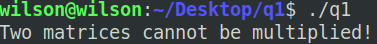
\includegraphics[width=0.5\textwidth]{output.png}
        \caption{Console output for Q1)b).}
    \end{figure}
    
    \item %Q2
    
    \begin{enumerate}
        
        \item \verb|final|, \verb|main.o|, \verb|block1.o|, \verb|block2.o|. Those four files are listed as targets in the makefile.
        
        \item Files that are regenerated: \verb|block1.o| and \verb|final|. Files such as \verb|block2.o| are not regenerated because they do not depend on \verb|block1.c|. 
        
        \item \verb|main.o| and \verb|final| will be regenerated. Running \verb|touch| will not overwrite the content but will update the timestamp. \verb|make| compares the timestamp and detects changes in \verb|main.c|. Hence \verb|make| regenerates \verb|main.o|, which is the target that directly depends on \verb|main.c|, and \verb|final|, which depends on \verb|main.o|, or depends indirectly on \verb|main.c|.
        
    \end{enumerate}
    
    \item %Q3
    
    Ignore the clock waveform. It should be one rising edge then stay at high level.
    
    \begin{figure}[ht]
            \centering
                \begin{wave}{2}{15}[h!]
                    \nextwave{a} \unknown{1} \bit{0}{2} \bit{1}{8} \bit{0}{5}
                    \nextwave{b} \unknown{13} \bit{1}{2} \bit{0}{1}
            \end{wave}
            \caption{Timing waveform for Q3)a). Please ignore the clock waveform.}
    \end{figure}
    
    \begin{figure}[ht]
            \centering
                \begin{wave}{2}{15}[h!]
                    \nextwave{a} \unknown{1} \bit{0}{1} \bit{1}{6} \bit{0}{8}
                    \nextwave{b} \unknown{2} \bit{0}{14}
            \end{wave}
            \caption{Timing waveform for Q3)b). Please ignore the clock waveform.}
    \end{figure}
    
    \item %Q4
    
    \begin{enumerate}
        
        \item Variables on the left hand side of an assignment statement, whether it is blocking or non-blocking, inside an always block, are meant to be changed when the items in the sensitivity list change. Their values ought to be preserved until the next change or next time when they are re-assigned values. Such requirement demand latches to be implemented to hold the state while still be able to change. Hence the variable type reg come into the play. Other variable type such as wire cannot hold the values.
        
        \item Assignment outside the always block should be continuous. The left hand side of the assignment statement outside an always block should change as soon as the right hand side changes, though delays may occur. Such change should not be restricted by any factors such as the sensitivity list.
        
        \item Different always blocks may have the same sensitivity list. Hence they may change at the same time. Race conditions may occur when multiple always blocks want to change the same variable of type reg at the same. Therefore such kind of practice is highly discouraged.
        
        \item The initial block sets the value of the reg variables. In real life, it is not possible to set the values of latches or registers before any signals arrive at such devices. Hence not synthesizable. The delay is not controllable. The delay is caused by many factors, including the propagation delay, or the logic processing delay. The length of the delay can vary due to factors such as temperature and the structure of the FPGA. Same Verilog code running on different FPGA devices can result in different delays. Hence delay is also not synthesizable. Both initial and delay can be usable in simulation however.
        
    \end{enumerate}
    
\end{enumerate}

\end{document}
